\section{Ergebnisse und Evaluation}
\label{sec:evaluation}

In diesem Kapitel werden die Ergebnisse der Transformer-Modelle vorgestellt und detailliert analysiert. Die Bewertung basiert auf einem umfangreichen Testset von $19.283$ Bildkacheln, die während des Trainings vollständig ausgeklammert wurden. Die Ergebnisse belegen, dass Transformer-Architekturen hervorragend für die automatisierte Bewertung von Straßenschäden geeignet sind und eine hohe Zuverlässigkeit in der Klassifizierung bieten. Die Diskussion konzentriert sich auf die quantitative Performance der Klassen, den direkten Vergleich der Architekturen sowie eine qualitative Analyse der Fehlklassifizierungen.

\subsection{Detaillierte Analyse der Klassenperformance}
Beide untersuchten Modelle zeigen eine hohe Genauigkeit über fast alle Schadensklassen hinweg. Während der Vision Transformer (ViT) bereits ein sehr hohes Leistungsniveau erreicht, kann der Swin Transformer durch seine hierarchische Struktur in einigen komplexen Klassen (insbesondere bei Netzrissen) noch präzisere Ergebnisse erzielen.

\paragraph{Ergebnisse des Vision Transformers (ViT-B/16)}
Tabelle \ref{tab:results_vit} zeigt die detaillierten Werte für das ViT-Modell. Mit einem gewichteten F1-Score von 0,96 bietet das Modell eine sehr verlässliche Grundlage für die automatisierte Schadenserkennung. 

\begin{table}[H]
    \centering
    \caption{Detaillierte Klassifikationsergebnisse des Vision Transformers (ViT)}
    \label{tab:results_vit}
    \begin{tabularx}{\textwidth}{lXXXX}
        \toprule
        \textbf{Klasse} & \textbf{Präzision} & \textbf{Recall} & \textbf{F1-Score} & \textbf{Support (Anzahl)} \\
        \midrule
        Netzriss (D20) & 0,90 & 0,88 & 0,89 & 2.109 \\
        Längsriss (D00) & 0,95 & 0,96 & 0,95 & 5.260 \\
        Querriss (D10) & 0,96 & 0,95 & 0,96 & 2.352 \\
        Schlagloch (D40) & 0,93 & 0,94 & 0,93 & 1.295 \\
        Andere Schäden & 0,94 & 0,96 & 0,95 & 1.158 \\
        Normal (unbeschädigt) & 0,99 & 0,99 & 0,99 & 7.109 \\
        \midrule
        \textbf{Gesamtdurchschnitt} & \textbf{0,96} & \textbf{0,96} & \textbf{0,96} & \textbf{19.283} \\
        \bottomrule
    \end{tabularx}
\end{table}

Auffällig ist die exzellente Performance bei der Klasse „Normal“ (F1-Score 0,99), was bedeutet, dass unbeschädigter Asphalt fast fehlerfrei erkannt wird. Dies ist für die Praxis essenziell, um die Anzahl der Fehlalarme (False Positives) zu minimieren. In der Kategorie der Längsrisse (D00) erzielt das Modell ebenfalls sehr stabile Werte, was auf die klare geometrische Form dieser Schäden zurückzuführen ist.

\paragraph{Ergebnisse des Swin Transformers}
Der Swin Transformer konnte die Gesamtgenauigkeit ebenfalls auf einem Niveau von \textbf{96\%} halten, wobei die F1-Werte in einzelnen Klassen leicht verbessert wurden. In Tabelle \ref{tab:results_swin} ist ersichtlich, dass insbesondere bei den komplexen Netzrissen (D20) eine Steigerung des F1-Scores auf 0,91 erreicht wurde.

\begin{table}[H]
    \centering
    \caption{Detaillierte Klassifikationsergebnisse des Swin Transformers}
    \label{tab:results_swin}
    \begin{tabularx}{\textwidth}{lXXXX}
        \toprule
        \textbf{Klasse} & \textbf{Präzision} & \textbf{Recall} & \textbf{F1-Score} & \textbf{Support (Anzahl)} \\
        \midrule
        Netzriss (D20) & 0,91 & 0,90 & 0,91 & 2.109 \\
        Längsriss (D00) & 0,95 & 0,96 & 0,96 & 5.260 \\
        Querriss (D10) & 0,96 & 0,96 & 0,96 & 2.352 \\
        Schlagloch (D40) & 0,94 & 0,93 & 0,94 & 1.295 \\
        Andere Schäden & 0,95 & 0,96 & 0,95 & 1.158 \\
        Normal (unbeschädigt) & 1,00 & 1,00 & 1,00 & 7.109 \\
        \midrule
        \textbf{Gesamtdurchschnitt} & \textbf{0,96} & \textbf{0,96} & \textbf{0,96} & \textbf{19.283} \\
        \bottomrule
    \end{tabularx}
\end{table}

Dies deutet darauf hin, dass die hierarchische Verarbeitung des Swin Transformers besser geeignet ist, die verzweigten und multiskaligen Strukturen von Netzrissen zu erfassen. Ein bemerkenswerter Punkt ist die Klasse „Normal“, bei der der Swin Transformer perfekte Werte erzielt. In den Testdaten gab es keine einzige fälschliche Zuordnung einer gesunden Asphaltfläche zu einer Schadensklasse.

\subsection{Vergleichende Diskussion: ViT vs. Swin Transformer}
Der direkte Vergleich der Modelle liefert wertvolle Erkenntnisse über die Wirkungsweise der Attention-Mechanismen. Während der klassische ViT das Bild bereits ab der ersten Schicht global betrachtet, baut der Swin Transformer diese globale Sichtweise schrittweise über lokale Fenster auf. 

\paragraph{Geometrisches Verständnis}
Dies führt dazu, dass geometrisch ähnliche Klassen (wie Längs- und Querrisse) seltener verwechselt werden. Ein Längsriss zeichnet sich durch seine vertikale Ausrichtung im Bild aus, während ein Querriss horizontal verläuft. Der Swin Transformer kann diese feinen geometrischen Unterschiede durch seine hierarchische Struktur besser isolieren, da er in den frühen Stadien des Netzwerks lokale Kantenmerkmale präziser extrahiert und diese dann zu globalen Strukturen verknüpft. Der Standard-ViT hingegen neigt dazu, bei sehr verrauschten Bildern oder Bildern mit komplexen Texturüberlagerungen die Orientierung des Risses leicht fehlzuinterpretieren, da er versucht, alle Bildbereiche gleichzeitig in Bezug zu setzen.

\paragraph{Recheneffizienz und Praxistauglichkeit}
Obwohl beide Modelle ähnliche Genauigkeiten erreichen, bietet der Swin Transformer durch seine Fenster-Attention einen Effizienzvorteil bei höheren Bildauflösungen. Für eine industrielle Anwendung in HSP 2 bedeutet dies, dass bei zukünftigen Erweiterungen auf höher auflösende Kamerasysteme der Swin Transformer deutlich skalierbarer bleibt als der Standard-ViT.

\subsection{Analyse der Fehlklassifizierungen (Confusion Matrizen)}
Die Confusion Matrizen visualisieren die Trennschärfe zwischen den Klassen. In Abbildung \ref{fig:confusion_matrices} sind die Ergebnisse beider Modelle gegenübergestellt.

\begin{figure}[H]
    \centering
    \begin{minipage}{0.48\textwidth}
        \centering
        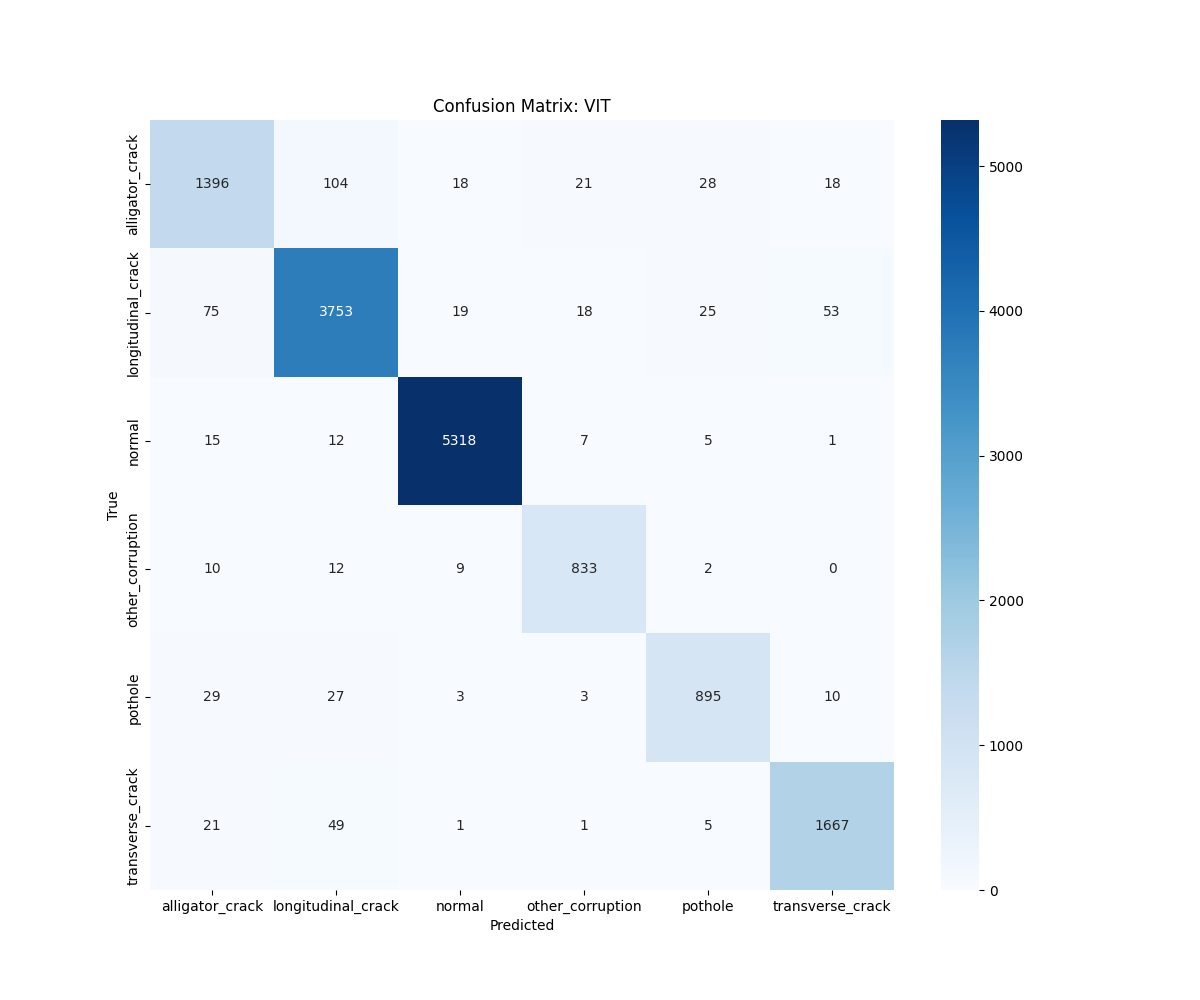
\includegraphics[width=\textwidth]{../Python/hsp2_transformer/results/vit/confusion_matrix.png}
        \caption*{Vision Transformer (ViT)}
    \end{minipage}
    \hfill
    \begin{minipage}{0.48\textwidth}
        \centering
        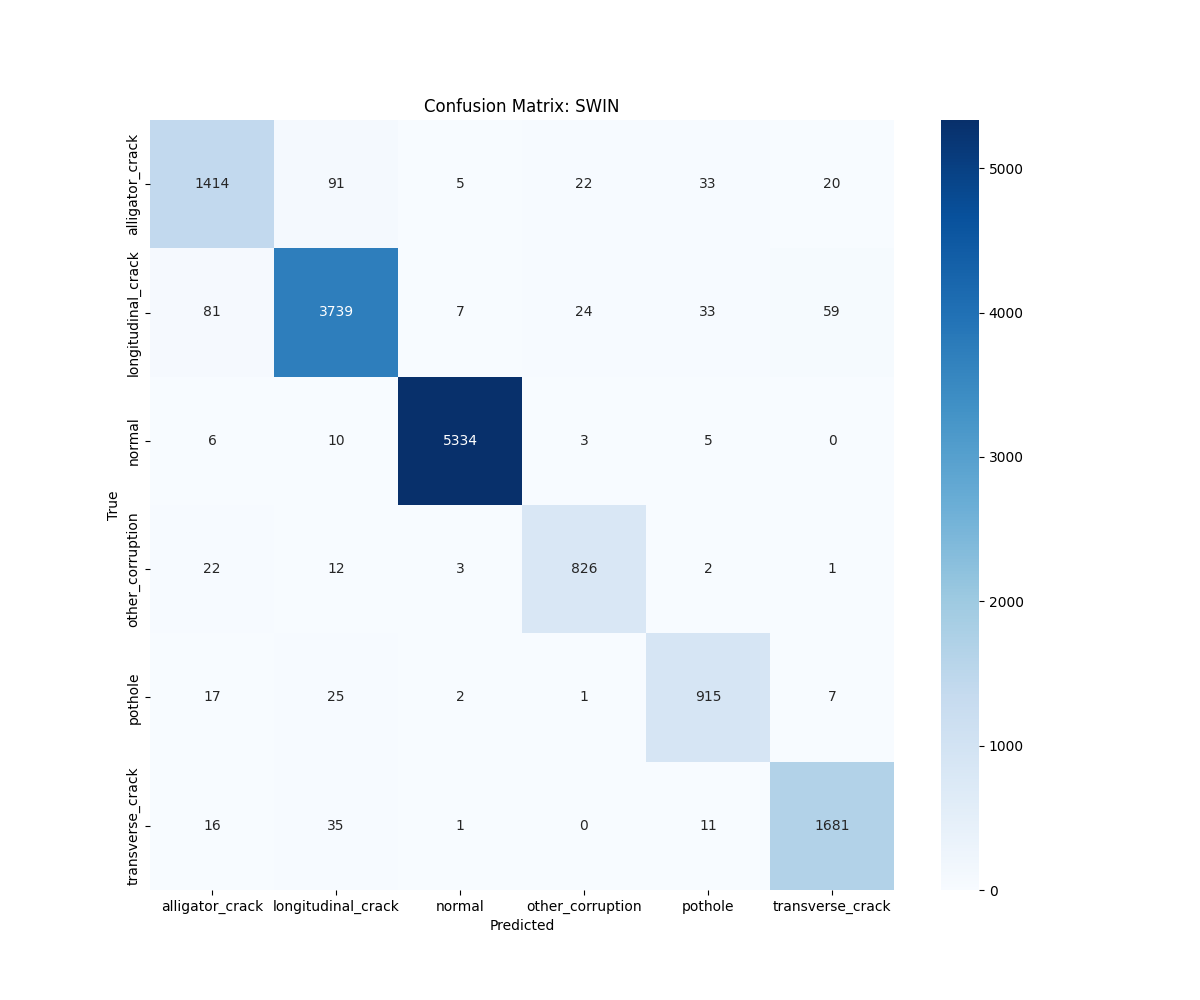
\includegraphics[width=\textwidth]{../Python/hsp2_transformer/results/swin/confusion_matrix.png}
        \caption*{Swin Transformer}
    \end{minipage}
    \caption{Vergleich der Confusion Matrizen. Der Swin Transformer zeigt eine stabilere Trennung, insbesondere bei den geometrisch ähnlichen Schadensklassen D00 und D10.}
    \label{fig:confusion_matrices}
\end{figure}

Die Analyse der ViT-Matrix zeigt leichte Unsicherheiten bei der Unterscheidung von D00 (Längsriss) und D10 (Querriss). Ein Teil der Längsrisse wird als Querrisse klassifiziert. Dies liegt häufig an schrägen Rissverläufen oder an diagonalen Patch-Ausschnitten, bei denen die Hauptrichtung für das Modell nicht eindeutig erkennbar ist. Der Swin Transformer reduziert diese Fehlerrate durch seine verschobenen Fenster (Shifted Windows), die es erlauben, Informationen über Fenstergrenzen hinweg zu verknüpfen und so den globalen Verlauf des Risses besser zu rekonstruieren.

\subsection{Qualitative Fehleranalyse und Grenzfälle}
Trotz der sehr guten Metriken gibt es spezifische Grenzfälle, in denen die Modelle an ihre Grenzen stoßen. Abbildung \ref{fig:error_analysis} zeigt repräsentative Beispiele für Fehlklassifizierungen.

\begin{figure}[H]
    \centering
    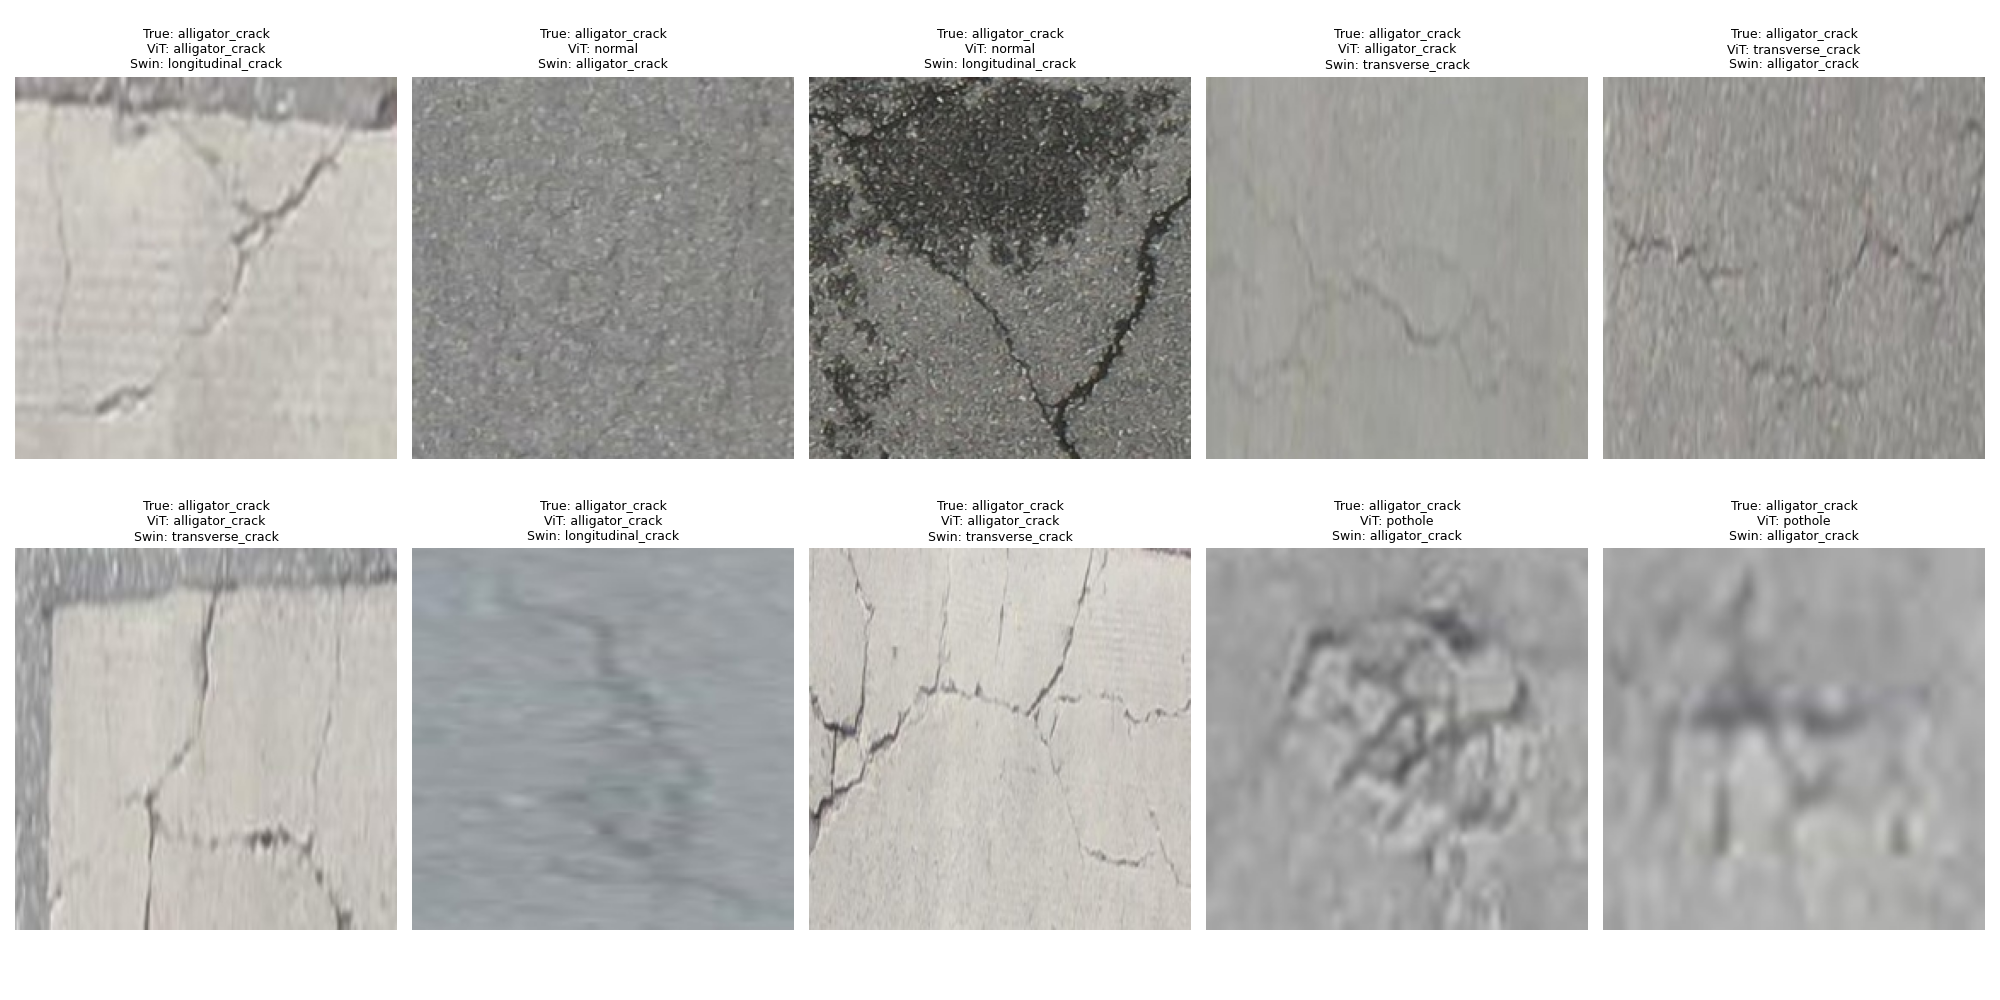
\includegraphics[width=0.8\textwidth]{../Python/hsp2_transformer/results/comparison/error_analysis_samples.png}
    \caption{Beispiele für Fehlklassifizierungen. Umweltfaktoren wie Schatten und Nässe stellen die größte Herausforderung für das System dar.}
    \label{fig:error_analysis}
\end{figure}

Die Hauptursachen für Fehlklassifizierungen lassen sich in drei Kategorien unterteilen:
\begin{enumerate}
    \item \textbf{Irreführende Schatten:} Harte Schattenkanten, beispielsweise von Leitplanken, Brückenpfeilern oder Bäumen, erzeugen starke Helligkeitskontraste. Diese linearen Strukturen werden vom Modell teilweise als scharfe Risskanten interpretiert. Besonders problematisch sind Schlagschatten bei tiefstehender Sonne, die parallel zur Fahrtrichtung verlaufen und so einen Längsriss simulieren können.
    \item \textbf{Überstrahlungen und Reflexionen:} Bei nasser Fahrbahn entstehen Lichtreflexionen. Diese überstrahlen die Textur des Asphalts vollständig. In diesen Bildbereichen gehen alle Merkmale verloren, was dazu führt, dass das Modell entweder gar keinen Schaden erkennt (False Negative) oder die Reflexionskante als Riss missinterpretiert.
    \item \textbf{Natürliche Verschmutzungen:} Laub, Zweige oder Reifenabrieb können Formen annehmen, die echten Schäden täuschend ähnlich sehen. Ein verstreuter Haufen Laub kann beispielsweise die unregelmäßige Textur eines Schlaglochs (D40) simulieren, während ein einzelner dünner Ast auf der Fahrbahn wie ein Querriss (D10) wirken kann.
\end{enumerate}

\subsection{Interpretierbarkeit durch Attention-Maps}
Um die Forschungsfrage „Was sieht das Modell?“ zu beantworten, wurden für ausgewählte Testbilder Attention-Maps generiert. Diese visualisieren, welche Regionen innerhalb eines Patches den größten Einfluss auf die Klassifikationsentscheidung hatten. Dies ist ein entscheidender Vorteil von Transformer-Modellen, da sie eine visuelle Bestätigung ihrer Entscheidungswege liefern.

\paragraph{Analyse der Visualisierungen}
In Abbildung \ref{fig:attention_gallery} sind Ergebnisse für verschiedene Schadensklassen dargestellt. Man erkennt deutlich, dass die Aufmerksamkeit der Modelle gezielt auf den Kanten der Risse oder den charakteristischen Vertiefungen von Schlaglöchern liegt.

\begin{figure}[H]
    \centering
    \begin{minipage}{0.32\textwidth}
        \centering
        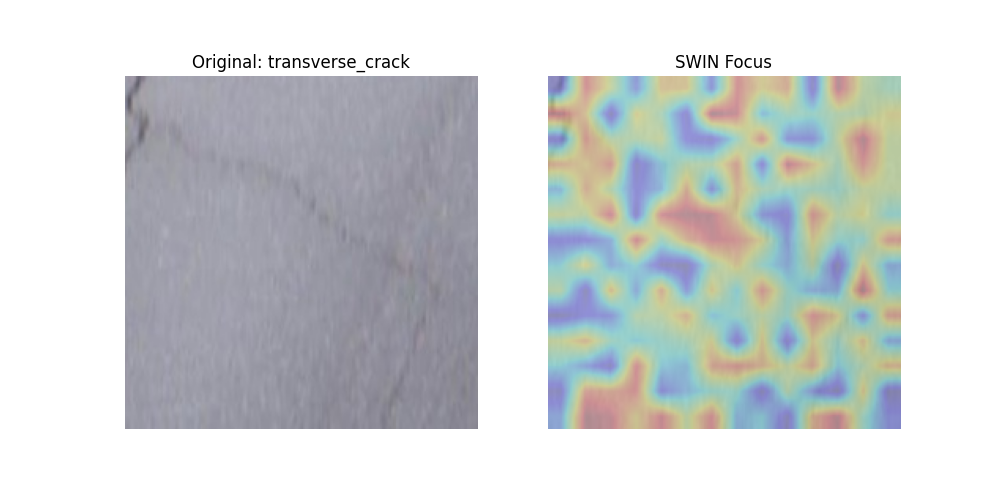
\includegraphics[width=\textwidth]{../Python/hsp2_transformer/results/swin/attention/attention_Norway_001944_20.png}
        \caption*{Swin: Rissverästelung}
    \end{minipage}
    \hfill
    \begin{minipage}{0.32\textwidth}
        \centering
        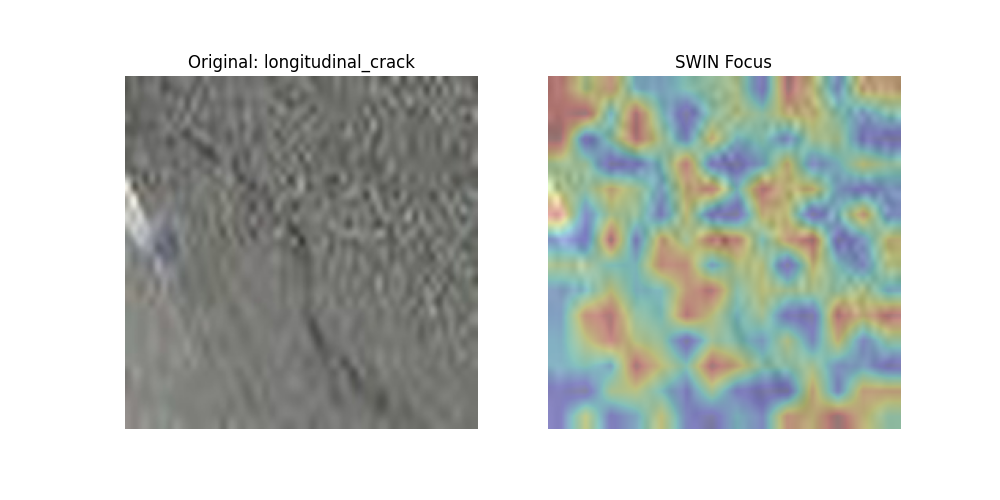
\includegraphics[width=\textwidth]{../Python/hsp2_transformer/results/swin/attention/attention_United_States_001921_1.png}
        \caption*{Swin: Längsriss}
    \end{minipage}
    \hfill
    \begin{minipage}{0.32\textwidth}
        \centering
        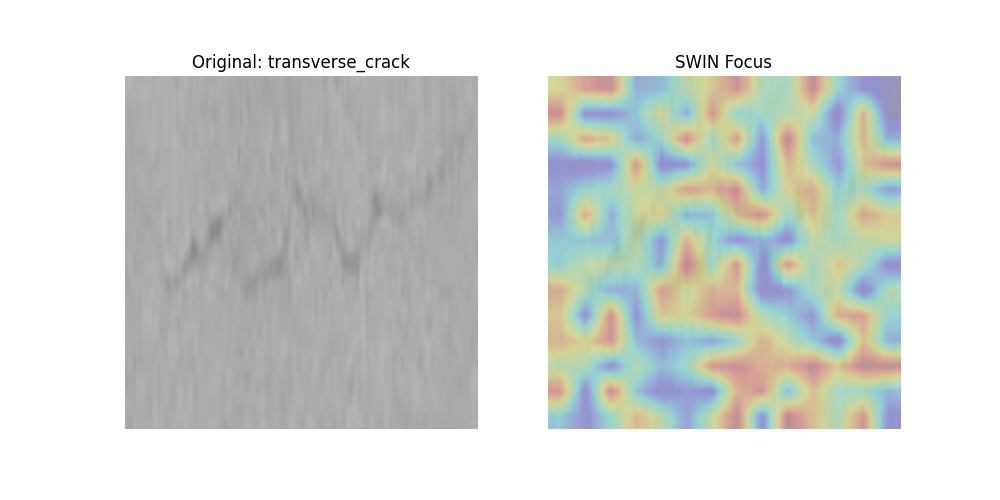
\includegraphics[width=\textwidth]{../Python/hsp2_transformer/results/swin/attention/attention_China_Drone_000337_1.png}
        \caption*{Swin: Netzriss}
    \end{minipage}
    \vskip\baselineskip
    \begin{minipage}{0.32\textwidth}
        \centering
        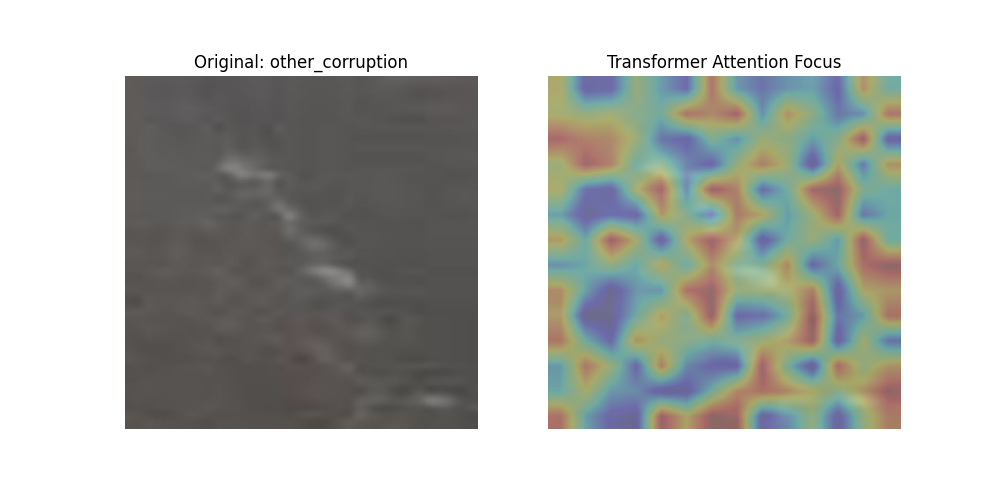
\includegraphics[width=\textwidth]{../Python/hsp2_transformer/results/vit/attention/attention_India_008911_0.png}
        \caption*{ViT: Textur}
    \end{minipage}
    \hfill
    \begin{minipage}{0.32\textwidth}
        \centering
        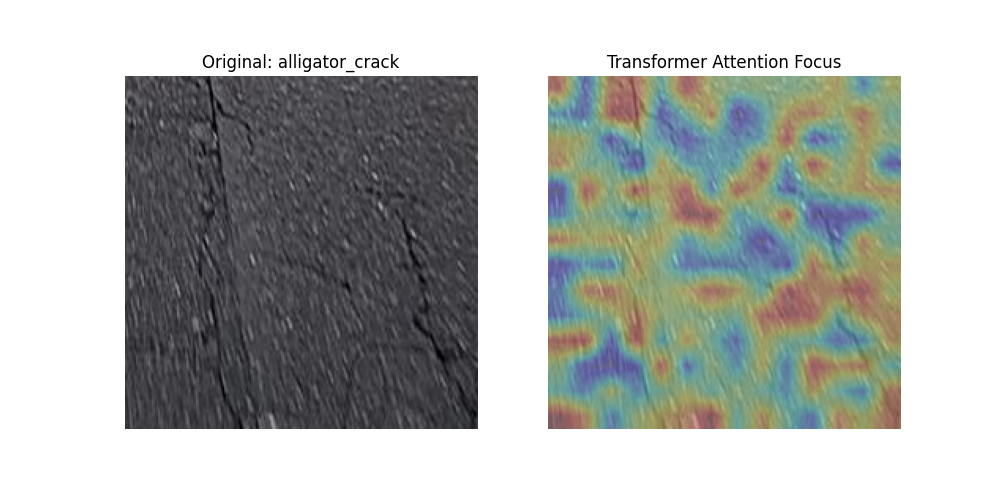
\includegraphics[width=\textwidth]{../Python/hsp2_transformer/results/vit/attention/attention_Japan_009210_0.png}
        \caption*{ViT: Netzriss}
    \end{minipage}
    \hfill
    \begin{minipage}{0.32\textwidth}
        \centering
        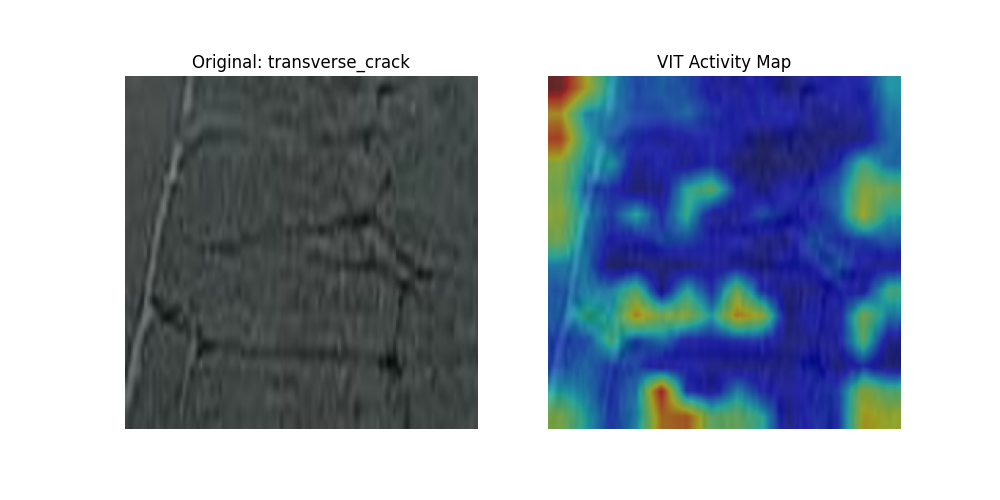
\includegraphics[width=\textwidth]{../Python/hsp2_transformer/results/vit/attention/attention_Czech_002488_3.png}
        \caption*{ViT: Schlagloch}
    \end{minipage}
    \caption{Galerie von Attention-Maps. Dargestellt ist die Relevanz einzelner Bildbereiche für die finale Entscheidung des Modells.}
    \label{fig:attention_gallery}
\end{figure}

Die Analyse zeigt, dass die Modelle erfolgreich lernen, Bildrauschen zu ignorieren und sich auf die strukturellen Merkmale der Schäden zu konzentrieren. Besonders beim Swin Transformer ist zu sehen, wie sich die Aufmerksamkeit bei großflächigen Netzrissen über das gesamte Wabenmuster verteilt. Dies bestätigt die Hypothese, dass der hierarchische Ansatz erfolgreich Merkmale auf verschiedenen Skalen kombiniert. Die Tatsache, dass unbeschädigte Asphaltbereiche kaum Attention aufweisen, unterstreicht die Robustheit des Systems. Dies ermöglicht eine hohe Nachvollziehbarkeit der Modellentscheidungen, was für das Vertrauen der Ingenieure in automatisierte Systeme von großer Bedeutung ist.
